\documentclass[12pt]{amsart}

% formatting stuff
\addtolength{\hoffset}{-2.25cm}
\addtolength{\textwidth}{4.5cm}
\addtolength{\voffset}{-2.5cm}
\addtolength{\textheight}{5cm}
\setlength{\parskip}{0pt}
\setlength{\parindent}{0pt}

% \usepackage{amsthm}
% \usepackage{amsmath}
\usepackage{amssymb}
\usepackage[colorlinks = true, linkcolor = black, citecolor = black, final]{hyperref}

\usepackage{graphicx}
\usepackage{multicol}
% \usepackage{ marvosym }
% \usepackage{wasysym}
% \usepackage{tikz}
% \usetikzlibrary{patterns}

\usepackage{listings}
\usepackage{xcolor}

\definecolor{codegreen}{rgb}{0,0.6,0}
\definecolor{codegray}{rgb}{0.5,0.5,0.5}
\definecolor{codepurple}{rgb}{0.58,0,0.82}
\definecolor{backcolour}{rgb}{0.95,0.95,0.92}

\lstdefinestyle{mystyle}{
    backgroundcolor=\color{backcolour},   
    commentstyle=\color{codegreen},
    keywordstyle=\color{magenta},
    % numberstyle=\tiny\color{codegray},
    stringstyle=\color{codepurple},
    basicstyle=\ttfamily\footnotesize,
    breakatwhitespace=false,         
    breaklines=true,                 
    captionpos=b,                    
    keepspaces=true,                 
    numbers=none,                    
    numbersep=5pt,                  
    showspaces=false,                
    showstringspaces=false,
    showtabs=false,                  
    tabsize=2
}
\lstset{style=mystyle}

\newcommand{\ds}{\displaystyle}

\setlength{\parindent}{0in}

\pagestyle{empty}

% ----------------------------
% end preamble
% -----------------------------

\begin{document}

{\scshape Math 131} \hfill {\scshape \large Assignment 2} \hfill {\scshape Luke Henderson}
\smallskip
\hrule
\bigskip

For the source code for the coding problems, see the attached Jupyter notebook, Matlab live script. Alternatively, the entire git repository  is attached as a zip archive, and is available \href{https://github.com/blackHat-Magic/Math-131-HW2}{on GitHub}. The comments in the code have been omitted here for brevity. They are present in the Jupyter notebook and Matlab live script.

\begin{enumerate}
\item\textbf{Problem Statement:} How many iterations would it take to find one of the roots of $f(x) := (x - 1)^2 - 1$ on the interval $[1, 3]$ the bisection method with an error smaller than $10^{-5}$? \\
The least upper bound of the absolute error for the bisection method on a given function after $n$ iterations is given by $|x_n - c| \leq \frac{b - a}{2^n}$, where $x_n$ is the prediction for the root at the $n$th iteration of the bisection method. Following this, we can solve for
\begin{align*}
10^{-5} & \geq \frac{3 - 1}{2^n} \\
10^{-5} \times 2^n & \geq 2 \\
2^n & \geq 2 \times 10^5 \\
nlog(2) & \geq log(2) + 5log(10) \\
0.30103n & \geq 5.30103 \\
n & \geq 17.60964 \\
n \in \mathbb{N} & \implies n = 18 \\
\end{align*} \\
However, if one were to perform the bisection method on this function on this interval, they would find that after the first iteration, the algorithm has found the exact root, meaning that technically in this instance, only one iteration was needed to get an absolute error of less than $10^{-5}$. \\
\bigskip

\item\textbf{Problem Statement:} Consider the equation $f(x) := x^2 - 2x - 3 = 0$ which has the roots $c_1 = -1$ and $c_2 = 3$. Using as interval $[a, b] = [0, 5]$, what is the approximation to $c_2$ using the bisection method after 3 iterations? \\
\texttt{bisection\_method(lambda x: x**2 - 2*x - 3, a=0, b=5, N=3)} \\
The approximation for $c_2$ using the bisection method after 3 iterations is $3.125$.
\bigskip

\item\textbf{Problem Statement:} Consider the equation $f(x) := x^2 - 2x - 8 = 0$ which has the roots $c_1 = -2$ and $c_2 = 4$. We would like to find a function so that the fixed point method $x_{n+1} = g(x_n)$ converges to the root $c_2 = 4$ for every point $x_0 \in [3, 5]$. Which $g(x)$ should we choose? \\
(a) $g(x) = 2 + \frac{8}{x}$ should be chosen because it converges the fastest. (b) converges to 0. Not only is this not the root we are looking for, it is not a root of $f(x)$ at all.  Similarly, (d) converges to $-2$ immediately, which, while it is a root, is not the root we are looking for. (c) does not converge at all. That leaves only (a), which converges quickly to $4$. \\
\bigskip

\item\textbf{Problem Statement:} Write a \texttt{MATLAB} function, called \texttt{bisection\_method} that takes as inputs a function, $f$, two numbers, $a$, $b$, an error tolerance \texttt{tol}, and a maximum number of iterations, $N$, and finds a root $c$ of $f$ in the interval $[a, b]$ using the bisection method. \\
\bigskip

\newpage
{\scshape Math 131} \hfill {\scshape \large Assignment 1} \hfill {\scshape Luke Henderson}
\smallskip
\hrule
\bigskip

\begin{multicols}{2}
    \lstinputlisting[language=Python, caption=Python]{../py/problem4.py}
\columnbreak
    \lstinputlisting[language=Matlab, caption=Matlab]{../m/problem4.m}
\end{multicols}

\newpage
{\scshape Math 131} \hfill {\scshape \large Assignment 1} \hfill {\scshape Luke Henderson}
\smallskip
\hrule
\bigskip

\begin{enumerate}
    \addtocounter{enumii}{2}
    \item\textbf{Problem Statement:} Use the code to solve $f(x) = (2x^3 + 3x - 1)cos(x) - x = 0$ on $[-1, 1]$, for an accuracy of $10^{-5}$. Discuss the results.
    \begin{enumerate}
        \item The number of iterations used was $18$.
        \item The absolute error was approximately $7.6294 \times 10^{-6}$.
        \item The expected rate of convergence for the bisection method can be expressed as $|x_n - c| \leq \frac{b - a}{2^n}$, where $n \in \mathbb{N}$. The big-O notation for this is $O(2^{-n})$.
        \item\begin{multicols}{2}
            \lstinputlisting[language=Python, caption=Python]{../py/problem4civ.py}
        \columnbreak
            \lstinputlisting[language=Matlab, caption=Matlab]{../m/problem4civ.m}
        \end{multicols}
        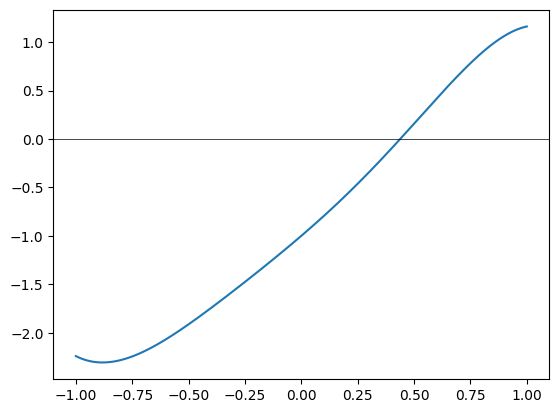
\includegraphics[scale=0.85]{../img/problem4civ.png} \\

\newpage
{\scshape Math 131} \hfill {\scshape \large Assignment 1} \hfill {\scshape Luke Henderson}
\smallskip
\hrule
\bigskip

        \item\begin{multicols}{2}
            \lstinputlisting[language=Python, caption=Python]{../py/problem4cv.py}
        \columnbreak
            \lstinputlisting[language=Matlab, caption=Matlab]{../m/problem4cv.m}
        \end{multicols}
        The number computed with the Python solver is approximately 0.43857, whereas the one computed with the bisection method is approximately 0.43856. I am not sure precisely which of the \href{https://docs.scipy.org/doc/scipy/reference/generated/scipy.optimize.root_scalar.html}{available solvers} in SciPy is used by default, but it is likely not the bisection method and instead a method that converges faster. That combined with the fact that there is no maximum iteration number by default means that the SciPy answer is likely closer to the answer. The fact that they vary by about $10^{-5}$ supports the idea that the early termination in \texttt{bisection\_method} contributes to the discrepancy, since that is the least upper bound for absolute error bound that was chosen.
    \end{enumerate}
\end{enumerate}
\bigskip

\item Write a \texttt{MATLAB} function, called \texttt{fixed\_point\_method} that takes as inputs a function, $g$, an initial guess $x_0$, an error tolerance, \texttt{tol}, and a maximum number of iterations, $N$, and outputs the fixed point of g, obtained using the fixed point method, starting with $x_0$. It should have an error defined by $E = |x_n - x_{n-1}|$, which is the absolute difference between the last two iterations, and stop when that error is less than the tolerance, or if the number of iterations exceeds $N$ - whichever happens first. use it to find the solution to the equation $x = e^{-x}$, with an accuracy of $10^{-10}$ for $x \in [-1, 1]$. State the initial guess, and how many iterations it took. Plot on the samge graph, $y = g(x)$ and $y = x$ using the `hold on' command.

\newpage
{\scshape Math 131} \hfill {\scshape \large Assignment 1} \hfill {\scshape Luke Henderson}
\smallskip
\hrule
\bigskip

\begin{multicols}{2}
    \lstinputlisting[language=Python, caption=Python]{../py/problem5.py}
\columnbreak
    \lstinputlisting[language=Matlab, caption=Matlab]{../m/problem5.m}
\end{multicols}

\texttt{fixed\_point\_method(lambda x: math.exp(x*-1, tol=1e-10))} \\
The initial guess was 0 and it took 42 iterations to converge to an absolute error of less than $10^{-10}$.

\newpage
{\scshape Math 131} \hfill {\scshape \large Assignment 1} \hfill {\scshape Luke Henderson}
\smallskip
\hrule
\bigskip

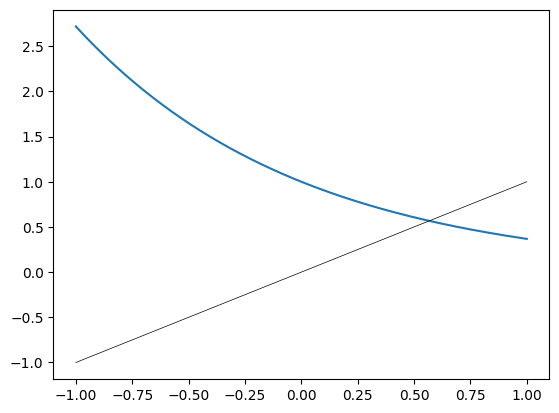
\includegraphics[scale=0.9]{../img/problem5.png} \\

\item \textbf{Problem Statement:} Write a \texttt{MATLAB} function, called \texttt{Newtons\_method} that takes as inputs a function $f$, its derivative, $f'$, an initial guess $x_0$, an error tolerance, $tol$, and a maximum number of iterations, $N$, and outputs the root of $f$ obtained uing Newton's method (denoted by $c$). It should stop when the upper bound for absolute error exceeds the error tolerance, or if the number of iterations exceeds $N$ - whichever happens first. \\
Use the function to find the root of the equation $arctan(x) = 1$ with an initial guess $x_0 = 2$, to an accuracy of less than $\texttt{tol} = 10^{-8}$. Did it converge? If so, in how many iterations? If not, why didn't it converge, and what happened-did it diverge, or end up in an infinite loop? Plot on the same graph the function and the eaxis $y = 0$. Test with $x_0 = -2$. What is happening?

\newpage
{\scshape Math 131} \hfill {\scshape \large Assignment 1} \hfill {\scshape Luke Henderson}
\smallskip
\hrule
\bigskip

\begin{multicols}{2}
    \lstinputlisting[language=Python, caption=Python]{../py/problem6.py}
\columnbreak
    \lstinputlisting[language=Matlab, caption=Matlab]{../m/problem6.m}
\end{multicols}

\newpage
{\scshape Math 131} \hfill {\scshape \large Assignment 1} \hfill {\scshape Luke Henderson}
\smallskip
\hrule
\bigskip

When finding the root of the equation $arctan(x) = 1$ using \texttt{Newtons\_method} using $x_0 = -2$, the function runs into an overflow error. What happens is that the method diverges; the derivative at the initial point is shallow enough to cause it to choose a new point on the next iteration that is much farther away. Because with $arctan$, the derivative gets closer to $0$ as $x$ gets farther away, the distance from the starting point keeps increasing, getting further and further away from the origin until $x_n$ is too large to be represented in the computer's memory. \\
Choosing $x_0 = 2$ allows the function to converge because the derivative at that point is steep enough to send the next iteration to a point closer to zero, allowing the method to converge.

\end{enumerate}

\end{document}